\documentclass[11pt,preprint,nocopyrightspace]{sigplanconf}
%
%% SOME OF OUR DEFINITIONS
%
\usepackage{xspace}
%\newcommand{\sys}{MiniCrypt\xspace}


\usepackage{fancyvrb}
\usepackage{listings}

\usepackage[compact]{titlesec}
%\titleformat{\section}{\normalfont\bfseries}{\thesection}{1em}{}
%\titlespacing*{\section}{1pt}{*0}{1pt}

\newcommand{\longerpaper}[1]{}

\usepackage{numprint}

\usepackage{multirow}

\lstset{
    basicstyle=\footnotesize\ttfamily,
      columns=fullflexible,
        keepspaces=true,
        }

\usepackage{subfigure}
\usepackage{ifpdf}
\usepackage[usenames,dvipsnames]{color}
\usepackage[letterpaper, breaklinks, pdfborder={0 0 0}]{hyperref}
\hypersetup{
    backref=true
      bookmarksnumbered,
        colorlinks=true,
          pdfstartview={FitH},
            citecolor={blue},
              linkcolor={blue},
                urlcolor={blue},
                  citecolor={blue},
                    pdfpagemode={UseOutlines}
                      }

  %\usepackage{algorithmic}

\usepackage[noend]{algpseudocode}

% edit the comments
\usepackage{eqparbox}
\renewcommand{\algorithmiccomment}[1]{\eqparbox{COMMENT}{// {\emph
      #1}}}

%\usepackage{multicol}
\usepackage{amsmath, amssymb}
\usepackage{amsthm}
\usepackage{enumitem}
%\usepackage{rotating}
%\onehalfspacing
%\newcommand{\tbd}[1]{[{\bf{#1}}]}
\newcommand{\tbd}[1]{}
\newcommand{\ie}{{\it i.e.}}
\newcommand{\eg}{{\it e.g.}}
\newcommand{\etc}{{\it etc.}}
\newcommand{\eat}[1]{}


\newcommand{\mypara}[1]{\noindent{\bf {#1}.}~}
\newcommand{\submypara}[1]{\medskip\noindent{\it {#1}.}~}
\newcommand{\chk}{$\checkmark$}
\newcommand{\dsh}{{\bf --}}
\newcommand{\til}{{\bf\large \textasciitilde}}
\usepackage{rotating}

\usepackage{framed}


% for packing
\newcommand{\mem}{\mathsf{MemorySize}\xspace}
\newcommand{\data}{\mathsf{Data}\xspace}
\newcommand{\cratio}{\mathsf{cr}\xspace}
\newcommand{\maxcr}{\mathsf{maxcr}\xspace}
\newcommand{\sizeof}{\mathsf{sizeof}\xspace}
\newcommand{\nmax}{n_{\max}}
\newcommand{\rowsize}{\mathsf{rowsize}}
\newcommand{\diskbw}{\mathsf{DiskTransferBandwidth}\xspace}
\newcommand{\diskseek}{\mathsf{DiskSeekTime}\xspace}


% RESULTS


\usepackage{enumitem}
\setlist[itemize]{itemsep=0.00cm}
\setlist[itemize]{parsep=0.01cm}
%\setlist[itemize]{parskip=0.01cm}


\newenvironment{myitemize}
{ \begin{itemize}[nolistsep]
        \setlength{\itemsep}{0.5pt}
            \setlength{\parskip}{0.9pt}
                \setlength{\parsep}{0.1pt}     }
{ \end{itemize}                  }

\newcommand{\green}[1]{{\color{ForestGreen}{#1}}}


% our encryption scheme

\newcommand{\keygen}{\mathsf{KeyGen}}
\newcommand{\Enc}{\mathsf{Enc}}
\newcommand{\enc}{\Enc}
\newcommand{\en}{\mathsf{enc}}


\renewcommand{\mod}{\mathsf{mod}\xspace}

% requires amsthm, enumitem
%\theoremstyle{algorithms}
%\newtheorem{construction}{Algorithm}
%\newcommand{\ALGORITHM}[4]{%  name, llabel, intro, \items
%\begin{construction}[#1]\label{#2} \mbox{}
%\normalfont\noindent
% #3
% \vspace{0.13\baselineskip}
% \begin{enumerate}[noitemsep,nolistsep]\itemsep=0.1\baselineskip
% #4
% \end{enumerate}
% \end{construction}
%}



\newcommand{\ALGORITHM}[4]{%  name, llabel, intro, \items
  \let\oldi\labelenumi
  \let\oldii\labelenumii
  \let\oldiii\labelenumiii
  \renewcommand{\labelenumi}{\arabic{enumi}: }
  \renewcommand{\labelenumii}{\arabic{enumi}.\arabic{enumii}: }
  \renewcommand{\labelenumiii}{\arabic{enumi}.\arabic{enumii}.\arabic{enumiii}:
  }
  \noindent \textbf{#1:} \label{#2}
  #3
   \vspace{0.13\baselineskip}
    \begin{enumerate}[noitemsep,nolistsep]\itemsep=0.1\baselineskip
       #4
       \end{enumerate}
     \let\labelenumi\oldi
     \let\labelenumii\oldii
     \let\labelenumiii\oldii
     }

%\newcommand{\subparagraph}{\paragraph}
%\usepackage[compact]{titlesec}

%\newcommand{\simplequote}[1]{\begin{quote}{\it{#1}}\end{quote}}

%\renewcommand\%bibname{}


%\usepackage[compact]{titlesec}
%\titlespacing{\section}{0pt}{0pt}{0pt}
%\titlespacing*{?command?}{?left?}{?beforesep?}{?aftersep?}[?right?]



\newcommand{\tickYes}{\checkmark}

% people
\newcommand{\ion}[1]{{\color{Red} IS: {#1}}}
\newcommand{\rachit}[1]{{\color{Red} RAg: {#1}}}
\newcommand{\rp}[1]{{\color{Red} RPo: {#1}}}
\newcommand{\frank}[1]{{\color{CarnationPink} FL: {#1}}} % :)
\newcommand{\wz}[1]{{\color{SkyBlue} WZ: {#1}}} % :)
\newcommand{\qu}[1]{{\color{Magenta}  {\bf Question:} {#1}}}
\newcommand{\warning}[1]{{\color{Red}{\bf Warning: #1}}}
\newcommand{\todo}[1]{{\color{Red} [todo: {#1}]}}

\newcommand{\aes}{\mathsf{AES}}
\newcommand{\encr}{\mathsf{enc\_r}}
%
\newcommand{\get}{\texttt{get}}
\newcommand{\delete}{\texttt{delete}}
\renewcommand{\put}{\texttt{put}\@\xspace}
\newcommand{\key}{\texttt{key}\xspace}
\newcommand{\val}{\texttt{value}\xspace}
\newcommand{\ver}{\texttt{version}\xspace}
\newcommand{\packID}{\texttt{packID}\xspace}
\newcommand{\pvalue}{\texttt{pvalue}\xspace}
\newcommand{\low}{\texttt{low}\xspace}
\newcommand{\high}{\texttt{high}}
\newcommand{\merge}{\texttt{merge}}
\newcommand{\msplit}{\texttt{split}}
\newcommand{\result}{\texttt{result}}
\newcommand{\pack}{\texttt{pack}\xspace}
\newcommand{\ts}{\mathsf{ts}}


% Compact itemize and enumerate.  Note that they use the same counters and                         
% symbols as the usual itemize and enumerate environments.                                         
\makeatletter
\def\compactify{\itemsep=3pt plus3pt \topsep=3pt plus3pt \partopsep=0pt
\parsep=0pt \leftmargin=1.3em}
\let\latexusecounter=\usecounter
\def\CompactItemize{%                                                                              
  \ifnum \@itemdepth >\thr@@\@toodeep\else
    \advance\@itemdepth\@ne
    \edef\@itemitem{labelitem\romannumeral\the\@itemdepth}%                                        
    \expandafter
    \list
      \csname\@itemitem\endcsname
      {\compactify\def\makelabel##1{\hss\llap{##1}}}%                                              
  \fi}
\let\endCompactItemize\endlist
\newenvironment{CompactEnumerate}
  {\def\usecounter{\compactify\latexusecounter}
   \begin{enumerate}}
  {\end{enumerate}\let\usecounter=\latexusecounter}
\makeatother



\begin{document}



%
% --- Author Metadata here ---
%\conferenceinfo{WOODSTOCK}{'97 El Paso, Texas USA}
%\CopyrightYear{2007} % Allows default copyright year (20XX) to be
%over-ridden - IF NEED BE.
%\crdata{0-12345-67-8/90/01}  % Allows default copyright data
%(0-89791-88-6/97/05) to be over-ridden - IF NEED BE.
% --- End of Author Metadata ---

\title{A Study on Deanonymizing Anonymous Social Networks}

% other title: or An encrypted and compressed key-value store \\
% Reconciling encryption and compression for key-value stores
% other paper names:  XZip, EncZip, Enczipt, CryptZip, CZip, EZip,
% Cryptar/CrypTar  (crypt+tar), Tarx, Tarc (tar +crypt), MiniCrypt



%
% You need the command \numberofauthors to handle the 'placement
% and alignment' of the authors beneath the title.
%
% For aesthetic reasons, we recommend 'three authors at a time'
% i.e. three 'name/affiliation blocks' be placed beneath the title.
%
% NOTE: You are NOT restricted in how many 'rows' of
% ``name/affiliations'' may appear. We just ask that you restrict
% the number of 'columns' to three.
%
% Because of the available 'opening page real-estate'
% we ask you to refrain from putting more than six authors
% (two rows with three columns) beneath the article title.
% More than six makes the first-page appear very cluttered indeed.
%
% Use the \alignauthor commands to handle the names
% and affiliations for an 'aesthetic maximum' of six authors.
% Add names, affiliations, addresses for
% the seventh etc. author(s) as the argument for the
% \additionalauthors command.
% These 'additional authors' will be output/set for you
% without further effort on your part as the last section in
% the body of your article BEFORE References or any Appendices.

%\numberofauthors{5} %  in this sample file, there are a *total*
% of EIGHT authors. SIX appear on the 'first-page' (for formatting
% reasons) and the remaining two appear in the \additionalauthors
% section.
%
\authorinfo{}

%\date{30 July 1999}
% Just remember to make sure that the TOTAL number of authors
% is the number that will appear on the first page PLUS the
% number that will appear in the \additionalauthors section.

\maketitle



\begin{abstract}
Over the last year, anonymous microblogging applications like Yik Yak, Whisper, and Secret gained popularity. These services spread messages to  contacts without including any authorship information. In this project, we wish to explore whether a moderately powerful third-party adversary, e.g., a government agency or a school administration, could deanonymize messages by simply participating in the network and knowing the underlying social graph.

We believed this might be possible due to a recent body of work on locating the patient-zero for a disease spreading over a graph. In our case,  corresponds to a message, and nodes  once they observe the message. Existing work assumes that the estimator can uniformly sample the graph to learn a subset of the infected nodes; given this, there exist strong guarantees and tractable methods for inferring an infection source.

We will discuss our experiences trying to replicate the results presented in the literature and apply these estimators to social networks. We have found deanonymization to be significantly more challenging than we previously believed, and our project has been largely been spent trying to understand why that is.infectedare diseasethe users
\end{abstract}

\section{Introduction}

Recently, there has been a rise in the number of anonymous social networks. Such social networks \todo{cite here} often promise users that they are able to post messages such that it is impossible to tell who sent what message. The propagated messages do not have 
Under such promises, anonymous social network users may be tempted to post relatively sensitive information. For example, a user may post messages disapproving a political candidate running for office. The candidate will then have incentive to track down the person who actually posted the message. In this project, we want to ask the question: \textbf{how easy is it for a \emph{moderately} powerful adversary to track down the true source of the message?}

In this project, we investigate the posed question by implementing multiple message source detection algorithms and testing these algorithms in a simulation setting on various types of graphs. We take ideas from other domains studying infection sources (i.e. identifying the patient zero of an infectious disease outbreak in a region) and apply those algorithms to the anonymous social network setting. 

We do not assume a very powerful adversary such as the NSA. Services like Secret actually utilize a centralized server to propagate the users' messages, and government agencies would have the power to either break into those centralized servers themselves, or have court orders to request for message sources directly. Instead, we consider an adversary who is only \emph{moderately} powerful, such as a school administrator or a dissenting political opponent. These adversaries do not have access to the centralized server, but they do have access to certain \emph{spies} within the social network. These spies listen passively for messages and intercept them. After a certain time has elapsed, the spies come together and use the collected information to find the true source of the propagation. The intercepted messages also contain the receiving timestamps, which are crucial for tracking down the source.

More specifically, we would like to answer two questions
\begin{enumerate}
\item How many spies within the network must an adversary have in order to effectively find the true source of the message?
\item How should an adversary select spies in order to maximize the probability of finding the sources of messages? 
\end{enumerate}

%We believe we can show through simulation that networks are susceptible to deanonymization by adversaries with limited power to create friendships and/or corrupt nodes.
We simulate the spread of messages over various networks in the presence of \emph{spy nodes}. Given a simulated message spread, we try to infer the true source from the spy nodes’ intercepted messages.  We vary attributes such as graph topology and size, the number and distribution of spy nodes, the probability of a node approving a message. We also utilize different estimation algorithms to attempt to infer the true source of the message. 


\section{Related Work}

\subsection{Anonymous Social Networks} 
Recent years have seen the rise of a new class of social network built upon anonymous microblogging.
Such networks, including Secret \cite{secret}, Whisper \cite{whisper}, and Yik Yak \cite{yikyak}, enable users to share short messages with their friends without including any authorship information in the metadata. 
Whenever a user `likes' an incoming message, that message passes to the user's friends.
Under this spreading pattern, messages propagate across the network like an epidemic.
While content on these social networks is anonymous to individual network users, service providers store all communications (and authorship information) on centralized servers.
The networks are therefore not anonymous to service providers themselves, as well as government agencies or hackers who obtain access to these centralized servers.
Our work considers a different adversary that is more powerful than a single user, but less powerful than a government agency or service provider.
%Because this class of social networks is relatively new, to the best of our knowledge, no existing research exists on deanonymizing them.

These social networks are not the gold standard for anonymous communication. In the rest of this section, we will discuss the state-of-the-art in anonymous broadcast communication, and explain why those methods have not gained traction outside the research community.
A wide swath of literature---spanning a few decades---considers the problem of communicating anonymously.
Much of this work focuses on \emph{point-to-point} communication, offering properties like sender anonymity, receiver anonymity, and/or sender-receiver unlinkability. 
Work in this area includes Chaum's mix-nets \cite{chaum1981untraceable}, Tor \cite{tor}, Tarzan \cite{tarzan}, Crowds \cite{reiter1998crowds}, and Herbivore \cite{goel2003herbivore}, just to name a few.
While this body of literature has been very impactful, it is different from our problem of interest.

We instead focus on approaches that enable anonymous \emph{broadcast} communication.
Chaum's seminal work on the dining cryptographers problem launched this area of study \cite{chaum88}.
The problem is as follows: a group of cryptographers goes out to dinner. After the meal, they want to learn if one of them has paid the check, without revealing who paid.
Chaum's solution, known colloquially as a DC-net, requires parties to share secrets with their neighbors and publish a function of those secrets. %requires each cryptographer to flip a coin (in private) with the individuals on his left and right. Each coin flip is hence observed by exactly two people.
%Then, each cryptographer publishes the XOR of the two observed coin flips; if cryptographer Alice paid the check, then instead of publishing the true XOR of her coin flips, she publishes the opposite (e.g., a 0 instead of a 1).
To learn the desired information, each cryptographer computes a function of all the published information. %If nobody paid the check, this bitwise sum will evaluate to 0; otherwise it will evaluate to 1.
DC-nets offer perfect anonymity, but they rely on some assumptions that may not realize in practice, such as the participants being honest, or only one individual communicating at once.

Chaum's work on DC-nets launched a great deal of study on robust, scalable, and anonymous broadcast communication. 
Some of this work focuses on developing new anonymity primitives, such as anonymous broadcast encryption \cite{libert2012anonymous, fazio2012outsider}.
Anonymous broadcast encryption aims to send an encrypted message such that only a subset of recipients can decrypt the message, but none of the recipients knows any of the other recipients' identities; in other words, it provides receiver anonymity.
%Classical broadcast encryption schemes require each recipient to know the entire set of intended recipients, which violates recipient anonymity; anonymous broadcast encryption aims to relax this constraint. 
This work is outside our scope, as we are interested in broadcast systems that provide \emph{sender} anonymity.


Another branch of work focuses on refining DC-nets to exhibit better efficiency or robustness properties against threats to protocol security or correctness \cite{waidner1989dining,golle2004dining,corrigan2010dissent}.
For instance, \cite{golle2004dining} proposes non-interactive DC-net constructions that identify misbehaving parties with high probability.
\cite{corrigan2010dissent} extends this work by proposing a DC-net with a \emph{shuffled send} primitive, which helps provide integrity, anonymity, and accountability within the network.
These proposed improvements to DC-nets are fairly efficient, but they are likely to face challenges at an Internet-wide scale.
Advances in the construction of DC-nets have led to various applications, including voting systems \cite{fujioka1993practical,van2010anonymous}, distributed storage \cite{freeHavenProject}, and even point-to-point anonymous messaging \cite{goel2003herbivore}.
The details of these schemes are not important to understanding our current work; the key take-away is that they all use ideas from DC-nets on a relatively small scale.
For instance, Herbivore \cite{goel2003herbivore} is a point-to-point messaging system that uses DC-nets to provide sender anonymity---but only within a small cluster of the network.
Using DC-nets to communicate across an entire network would be massively impractical, due to their vulnerability to Sybils, Byzantines, and denial-of-service attacks.

The body of anonymous broadcast research has not yet found its way into a large-scale, widely-adopted social network. 
Several factors might explain this, including the scalability and security challenges we mentioned, as well as the difficulty of monetizing truly anonymous services.
The end result is that commercial anonymous social networks described earlier, such as Secret and Whisper, have built significant user bases while offering fairly weak anonymity properties.
As such, they present a juicy target for adversaries hoping to learn people's sensitive secrets.
In this work, we study exactly how powerful an adversary must be to deanonymize such a network.

\subsection{Deanonymizing Social Networks}

Researchers have worked on different techniques for deanonymizing social networks. Early approaches on user deanonymization~\cite{novak2004anti,narayanan2006break} come from inferring user identify from public messages sent by these users. For example, an early work~\cite{novak2004anti} analyzed pseudonymous posts on online bulletin boards. The paper uses machine learning techniques and data mining to analyze these posts. These algorithms extract features and detect post similarity, therefore inferring that some aliases are being used by the same user. 

A more sophisticated approach~\cite{backstrom2007wherefore} considers what happens when you have more limited information, such as only information regarding node connections. The paper models the network as a list of nodes and edges. Nodes are anonymized (original IDs replaced with new IDs), while the communication links (graph edges) are preserved. The attackers have a list of target nodes that they wish to compromise.
The attacks presented in this paper assume that the attackers can construct new nodes a network graph $G$ before it is anonymized. These fake nodes attempt to communicate with a list of targeted honest nodes and these communications are recorded as edges. After the graph is anonymized, the attackers will attempt to identify the fake nodes along with the targeted nodes. 
The aim of our project is a little different. We are attempting to deanonymize an online network that is already anonymized to a certain extent when the attack begins. A subset of the nodes in the network are assumed compromised, and the attackers will leverage anonymous messages to reconstruct the social network graph as well as re-identifying nodes. 

One recent~\cite{narayanan2009anonymizing} approach focuses on deanonymizing large scale social networks by developing a very generic re-identification algorithm. Social graph anonymizaion usually consists of releasing some partial information on a \emph{sanitized} version of the graph. 
The attackers are assumed to know some auxiliary information about the original graph $S$. This auxiliary information, designated as $S_{AUX}$, is a different network such that $S_{AUX}$ and $S$ partially overlap. Using the auxiliary information, the attackers can use an algorithm to deanonymize the sanitized version of $S$, $S_{SAN}$.
The algorithm consists of two steps, seed identification and propagation. Seed identification attempt to find a small amount of users that are present both in the anonymized network and the auxiliary graph. The propagation stage is an iterative process that finds new mappings between $S_{SAN}$ and $S_{AUX}$. This paper's analysis is very informative, and the generic algorithm is very applicable. However, it does not attempt to address the issue of tracking specific messages back to their original sources. We attempt to address both the network graph deanonymization (such that it is possible to discover the network connectivity) and the message deanonymization (such that it is possible to find the original source of the message). In addition, we would like to analyze and quantify the extent of the deanonymization spread for different network topology.

\subsection{Identifying a Rumor Source}
Here we discuss work on statistical rumor source inference over graphs; this literature will inform our choice of inference algorithms for identifying the source of a message.
Rumor source inference has been of interest for a long time, but a recent surge of statistical research started with Shah and Zaman \cite{shah2011rumors}. The problem is as follows: An infection is propagating over a graph according to a diffusion random process. 
That is, each infected node infects an uninfected neighbor in an exponentially-distributed amount of time.
Given the underlying graph structure and a single snapshot of the infection pattern at a given time, can the ``patient-zero" be inferred?
The authors propose a metric called \emph{rumor centrality}, which describes the centrality of a node in the infected subgraph.
They present an efficient method for computing rumor centrality and show that when the underlying social network is tree-structured, the node with maximum rumor-centrality is the true patient-zero with high probability. The intuition is that regular, symmetric spreading patterns (like diffusion) tend to place the true source in the center of the infection graph with high probability. 

Subsequent work has examined many variants of this problem. Examples include considering more general graph structures \cite{shah2012rumor} and altering the estimator's data-collection strategy \cite{pinto,karamchandani2013rumor,luo2013identify}.
In these last papers, the estimator samples a subset of infected nodes, and learns the timestamp at which each node first received the infection. 
This is equivalent to our notion of placing ``spies" in the network. 
This follow-up work mainly reinforces the point that under a variety of graph structures and information collection methods, rumor centrality and other heuristic centrality measures can consistently identify the source with high probability. 
These heuristics are therefore good candidates for our own inference problem. 
Another class of research instead develops new estimation techniques based on message-passing \cite{lokhov2014inferring} and spectral methods \cite{fioriti2012predicting}.
Although these methods perform well, their added complexity makes them less well-suited to our purposes.

While this body of work informs our choice of estimators for rumor source identification, it is not guaranteed that these estimators will work well. 
Existing research assumes that samples are taken regularly over the graph. 
In our work, these sampled nodes correspond to spies or Sybil nodes, which exhibit very different topological characteristics than normal social graph nodes \cite{narayanan2009anonymizing}.
The question is whether irregularly-spaced Sybil nodes (which are easy to make) can achieve the same deanonymization accuracy as a uniformly-spaced network of spies (which is difficult to build).


\section{Methodology}

\subsection{Model}

We assume an application model that is similar to Secret~\cite{secret}.
\begin{figure}
\centering
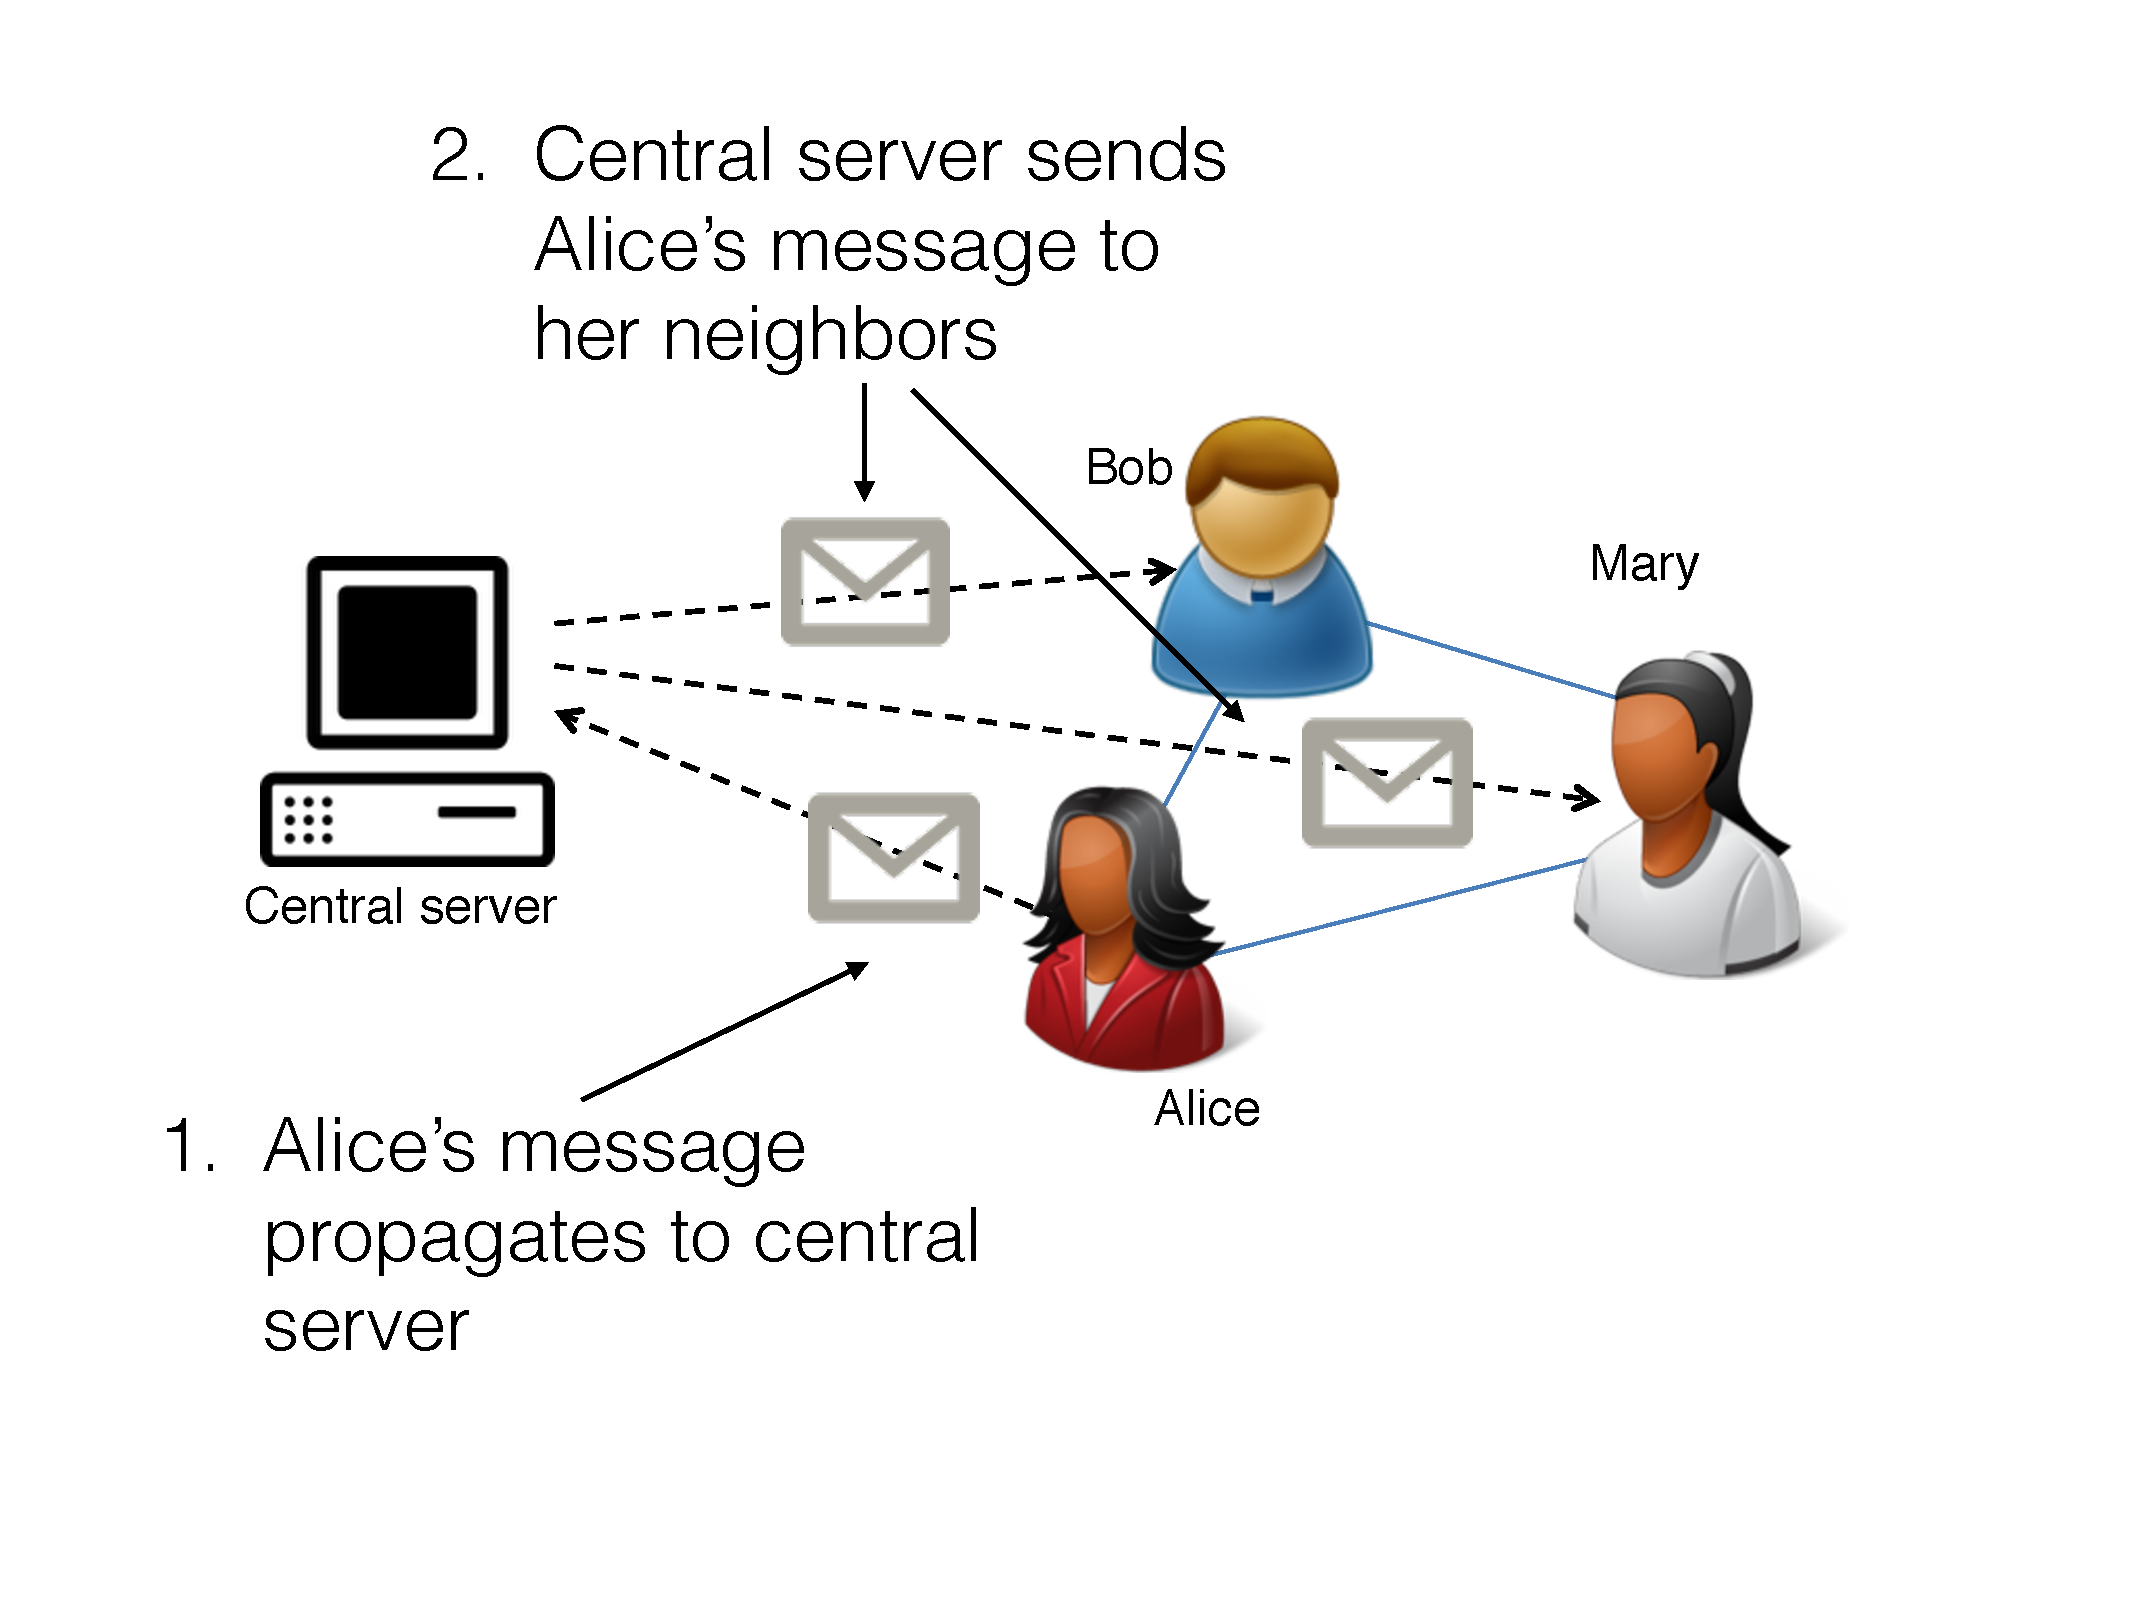
\includegraphics[height = 2.4in]{figures/secret_infrastructure}
\caption{An overview of the infrastructure for a typical anonymous social network.}
\label{fig:secret_infrastructure}
\end{figure}
Fig.~\ref{fig:secret_infrastructure} shows how a typical anonymous microblogging network works. Users are connected to friends as in a regular social network; we model this social network as a graph $\mathcal G(V,E)$, where $V$ denotes the set of vertices, or participants, in the network, and $E$ denotes the set of edges. When a source node, Alice, decides to send a message to her friends, her message is routed to a centralized server first. We denote the source node by $v^*$. The server propagates the message to Alice's neighbors, $\mathcal N(v^*)$. Alice's neighbors do not know who sent or authored the message. %To them, the message is from the centralized server instead of directly from Alice, and does not have any information about the sender herself. 
If one of Alice's friends decides to ``like'' the message, the message will be further propagated to her friend's friends. Thus, whenever a user receives a message, he/she does not know if a neighboring friend sent it, or if it was simply liked by a friend. We assume that propagation occurs with some time delay, which captures the time between the server pushing a message and the receipient actually seeing it. We model the delay between a user $i$ liking a message and the user's friend $j$ seeing the message as a random variable $\theta_{ij}$; the $\theta_{ij}$'s, or delays across each edge in the social graph, are assumed to be iid random variables. We do not specify the distribution of $\theta_{ij}$ \emph{a priori}; in principle, this should be informed by measurements of real social network usage.

Our adversarial model considers a moderately powerful adversary that is able to compromise certain users in the social network. This might occur by offering incentives to users and recruiting them to act as spies. The spies are not active, but are instead passive observers. The only thing that differentiates spies from honest users is that spies collect all observed messages (along with timestamps), and then send this information to the adversary. The adversary uses the collected message timetamps to attempt to track down the perpetrator of the message.
We assume there are $K$ spies in the network, $o_1,\ldots,o_K$. For a given message $m$, each spy $o_i$ will collect the timestamp $t_i^{(m)}$ at which it first receives the message. The adversary must then output an estimate $\hat v$, which it believes to be the true source of message $m$. %Therefore, the 

The central adversary will receive different sets of messages, and it will need to group them into a \emph{collection} -- a group of messages received at different nodes that came from the same source. We assume that these messages are not encrypted, and thus the adversary can use the plaintext information directly to identify the correct collection membership. 

\subsection{Efficacy of deanonymization}

We study the ability of this adversary to deanonymize users through simulation. A number of factors could impact deanonymization:

\begin{description}
\vspace{-0.1in}
\item[Underlying graph structure:] The underlying graph structure can significantly affect deanonymization. For example, a tree-like structure with no loops is easier to deanonymize because there are fewer possible paths between nodes to analyze. In our simulation, we study a range of graph structures, including trees, Erdos-Renyi, and Barabasi-Albert graphs.
\item[Fraction of spies:] The fraction of spies will greatly impact the deanonymization performance. Fewer spies means less information, and thus makes the true source much harder to track. Using simulation, we want to \emph{quantify} how many spies are needed to efficiently find the true source.
\item[Location of spies:] We hypothesize that selecting spies as high-degree nodes will increase the probability of detection, as popular nodes are more likely to see and propagate the message. However, this may be unrealistic in practice, as popular individuals (i.e., high-degree nodes) may hold more social leverage and may therefore resist recruitment attempts. A uniform distribution of spy nodes seems feasible for an adversary with moderate but limited resources. 
\item[Propagation latency:] The propagation latencies $\theta_{ij}$ are likely to depend on many factors, such as the popularity of the social network, the habits of its users, and the application platform (e.g., mobile vs. desktop).
In simulation, we model the propagation latency in two ways: using a Gaussian distribution with a high mean-to-standard-deviation ratio, and a geometric random variable. 
\item[Estimator:] To optimize probability of detection, i.e. $P(\hat v=v^*)$, the adversary would like to use a maximum-likelihood (ML) estimator. However, ML estimators are not known for general graph structures and propagation delay models. We therefore try different methods of estimation. The majority of our effort goes towards adapting the observer model~\cite{pinto} to our spy nodes setting.
\end{description}

\subsection{Estimators}
Initially, we attempted to come up with some estimators on our own. \todo{Should we mention the Jordan estimators here?}



\subsubsection{ML estimator for trees}
The observer model estimator~\cite{pinto} is a maximum likelihood estimator. The setup is quite similar to our simulation: given a graph $\mathcal G$, there exists a set of $K$ observers that observe information transmitted in the network. The collected information has a timestamp, as well as direction information (e.g. observer $o$ receives the message from neighbor $v$). This is the main difference between \cite{pinto} and our work; we do not assume that spies have direction information. \cite{pinto} also assumes that propagation delays are modeled by iid Gaussian random variables with distribution $\mathcal N(\mu,\sigma^2)$. We start by defining some terms:

Let $\boldsymbol{d}$ be the timestamp differences of observed arrivals with respect to some reference spy node, defined as
\begin{equation}
  \boldsymbol{d}_k = t_{k} - t_1
\end{equation}
where $t_i$ denotes the observed timestamp at spy $i$, and $k = 2,\ldots, K$.

The next term is the expected delay, which is the delay that one \emph{should} observe if the information had propagated from some candidate source $s$ ($s$ is an honest node in the graph):
\begin{equation}
  \boldsymbol{\mu}_{s,k} = \mu (|P(s, o_{k+1})| - |P(s, o_1)|)
\end{equation}
where $|P(u, v)|$ denotes the number of edges on the path that connects nodes $u$ and $v$. Finally, we define a scaled covariance matrix, which represents the covariance of the jointly-gaussian delay random variable:
\begin{equation}
  \boldsymbol{\Lambda}_{k, i} = \begin{cases}
    |P(o_1, o_{k+1})| & \text{if $k = i$} \\
    |P(o_1, o_{k+1}) \cap P(o_1, o_{i+1})| & \text{if $k \neq i$}.
  \end{cases}
\end{equation}
The authors use these terms to construct a source estimator for general trees:
\begin{equation}
\label{eq:general}
\hat{s} = \arg\max_{s \in \mathcal T_{a}} \dfrac{\exp(-\frac{1}{2} (\boldsymbol{d} - \boldsymbol{\mu}_{s})^{T} \boldsymbol{\Lambda}_s^{-1} (\boldsymbol{d} - \boldsymbol{\mu}_s) }{|\boldsymbol{\Lambda}_s|^{1/2}}.
\end{equation}

$\mathcal T_a$ denotes the \emph{pruned} tree. Pruning refers to the process of removing nodes that could not have possibly generated the observed information. For instance, consider the following 

Equation \ref{eq:general} can be applied to general graphs as a heuristic estimator. However, if the underlying graph is tree-structured, equation \ref{eq:general} simplifies to
\begin{equation}
\label{eq:tree}
\hat{s} = \arg\max_{s \in \tau_{a}} \boldsymbol{\mu}_{s}^{T} \boldsymbol{\Lambda}^{-1} (\boldsymbol{d} - \frac{1}{2}\boldsymbol{\mu}_s).
\end{equation}
because $\Lambda_s$ is constant for all candidate nodes. This estimator is provably optimal for tree-structured graphs.

\subsubsection{Nearest-spy estimator}
We also tested a heuristic estimator, which does not make use of the full available information. This estimator considers the first spy to receive the message. Without loss of generality, assume that spy is $o_1$. The estimator chooses an honest neighbor of that spy uniformly at random, and uses that as the estimate $\hat s$. This estimator does not use direction information. A trivial extension to this estimator uses direction estimation and picks $\hat s$ as the node that delivered the message to the first spy. We use this directionality information in comparing our results with those of \cite{pinto}, which make use of direction information.
\section{Evaluation}
\label{sec:eval}

The evaluation of our work is executed on a discrete-event simulator written in Python. This simulator is similar to existing discrete-event simulators such as ns3. Events are put onto a priority queue ordered by time, and executed in a single loop.

This simulator takes in as input different network structures with a list of nodes, links, and node types. 
Nodes can be either honest or malicious. As mentioned before, we simulate passive adversaries: malicious nodes are honest-but-curious. Whenever a malicious node receives a message, it adds the message, along with the time at which the message is received, to a list of intercepted messages. The timestamp used is the global simulator time, thus we assume that the spies' clocks are roughly synchronized (or that the synchronization time is much smaller than). 

At the start of a simulation run, a certain percentage of the nodes are compromised. The percentage number can be tweaked to adjust the number of malicious nodes in the network. The simulator then runs for some number of time steps and produces a list of messages intercepted from malicious nodes. After the simulation, the estimators take in the list of timestamped messages and produce guesses for the true source of the message.

\subsection{Estimator validation}
We started by attempting to replicate the estimator results in \cite{pinto}. 
In this replication process, we encountered four primary mistakes or omissions in \cite{pinto} that affected our estimation accuracy; some of these were easy to correct once we identified them, others were not. All equation numbers in this list are with respect to \cite{pinto} and the corresponding supplementary materials.
\begin{enumerate}
\item There is a typo in equation (2), which describes how to compute the observed delay vector. It should say $[\boldsymbol d]_k=t_{k+1}-t_1$ instead of $[\boldsymbol d]_k=t_{k+1}-t_k$. This is a small but important typo in the description of the estimator that leads to incorrect likelihoods. 
\item Algorithm 2 of the supplemental materials describes how to compute likelihoods for general graphs. In step 6, it should say ``compute the source likelihood using equation (4) for node $s$.", rather than ``using equation (7)." This is because over general graphs, the covariance matrix $\Lambda_s$ is not identical for all nodes, which causes the simplifications in equation (7) to be invalid. As such, the likelihoods should be computed using the more general equation (4). This error initially led to incorrect likelihood computations in our code.
\item Algorithm 2 of the supplemental materials does not explain how to prune graphs that are not tree-structured. Additionally, it does not describe how to incorporate the direction of infection into estimation. These omissions collectively have a significant impact the likelihoods obtained by the algorithm, and we suspect this is partially responsible for our inability to exactly reproduce their results.
\item The parameter specifications of the random graphs in Table 1 are not given. Specifically, the Barabasi-Albert parameter is not given. We therefore tried a range of different parameters.
\end{enumerate}
For point 3, the corresponding author of \cite{pinto} sent us part of his simulation code two days before the project due date, so we have revised our discussion to reflect what we learned from reading his code. Namely, his code helped explain how they prune graphs that are not tree-structured. 

For general graphs, pruning takes place in two steps: 1) For each spy node, remove all graph edges that were not used to transmit the message to the spy. 2) Step 1 will leave the graph disconnected; keep the connected component that contains the spy with the earliest timestamp. The resultant subgraph is called $\mathcal G_a$, and the optimization in equation \ref{eq:general} occurs as normal over the honest nodes of $\mathcal G_a$ (rather than $\mathcal T_a$). 

On a tree, this pruning procedure corresponds to only using timestamps from the nearest spies; if two spies lie on the same path (as defined by the direction of message transmission), then the latter spy's information will be discarded. For example, in Figure \ref{fig:pruning}, $o_2$'s timestamp $t_2$ would be discarded, because the edge between $o_1$ and $o_2$ would be cut. This is a reasonable approach, because conditioned on $o_1$'s information, $t_2$ is independent and therefore cannot improve the estimate. 

However, on a loopy graph, this approach discards viable message paths, thereby placing undue weight paths that might otherwise have a very low likelihood. For example, consider the graph in Figure \ref{fig:pruning2}. Even though the most likely path for the message is $0\rightarrow o_1\rightarrow 3 \rightarrow o_2$, pruning removes the edge between $o_1$ and node $3$, so the estimator acts as if the message traversed the path $0\rightarrow 4\rightarrow 5 \rightarrow 6 \rightarrow 7 \rightarrow 3 \rightarrow o_2$---a path with comparatively low likelihood. Although this pruning approach is not strictly correct, we will demonstrate that it performs well in practice. Indeed, our simulation results suggest that the high accuracy levels reported in \cite{pinto} over general graphs are mostly due to pruning, not the proposed estimator.
\begin{figure}[h]
\centering
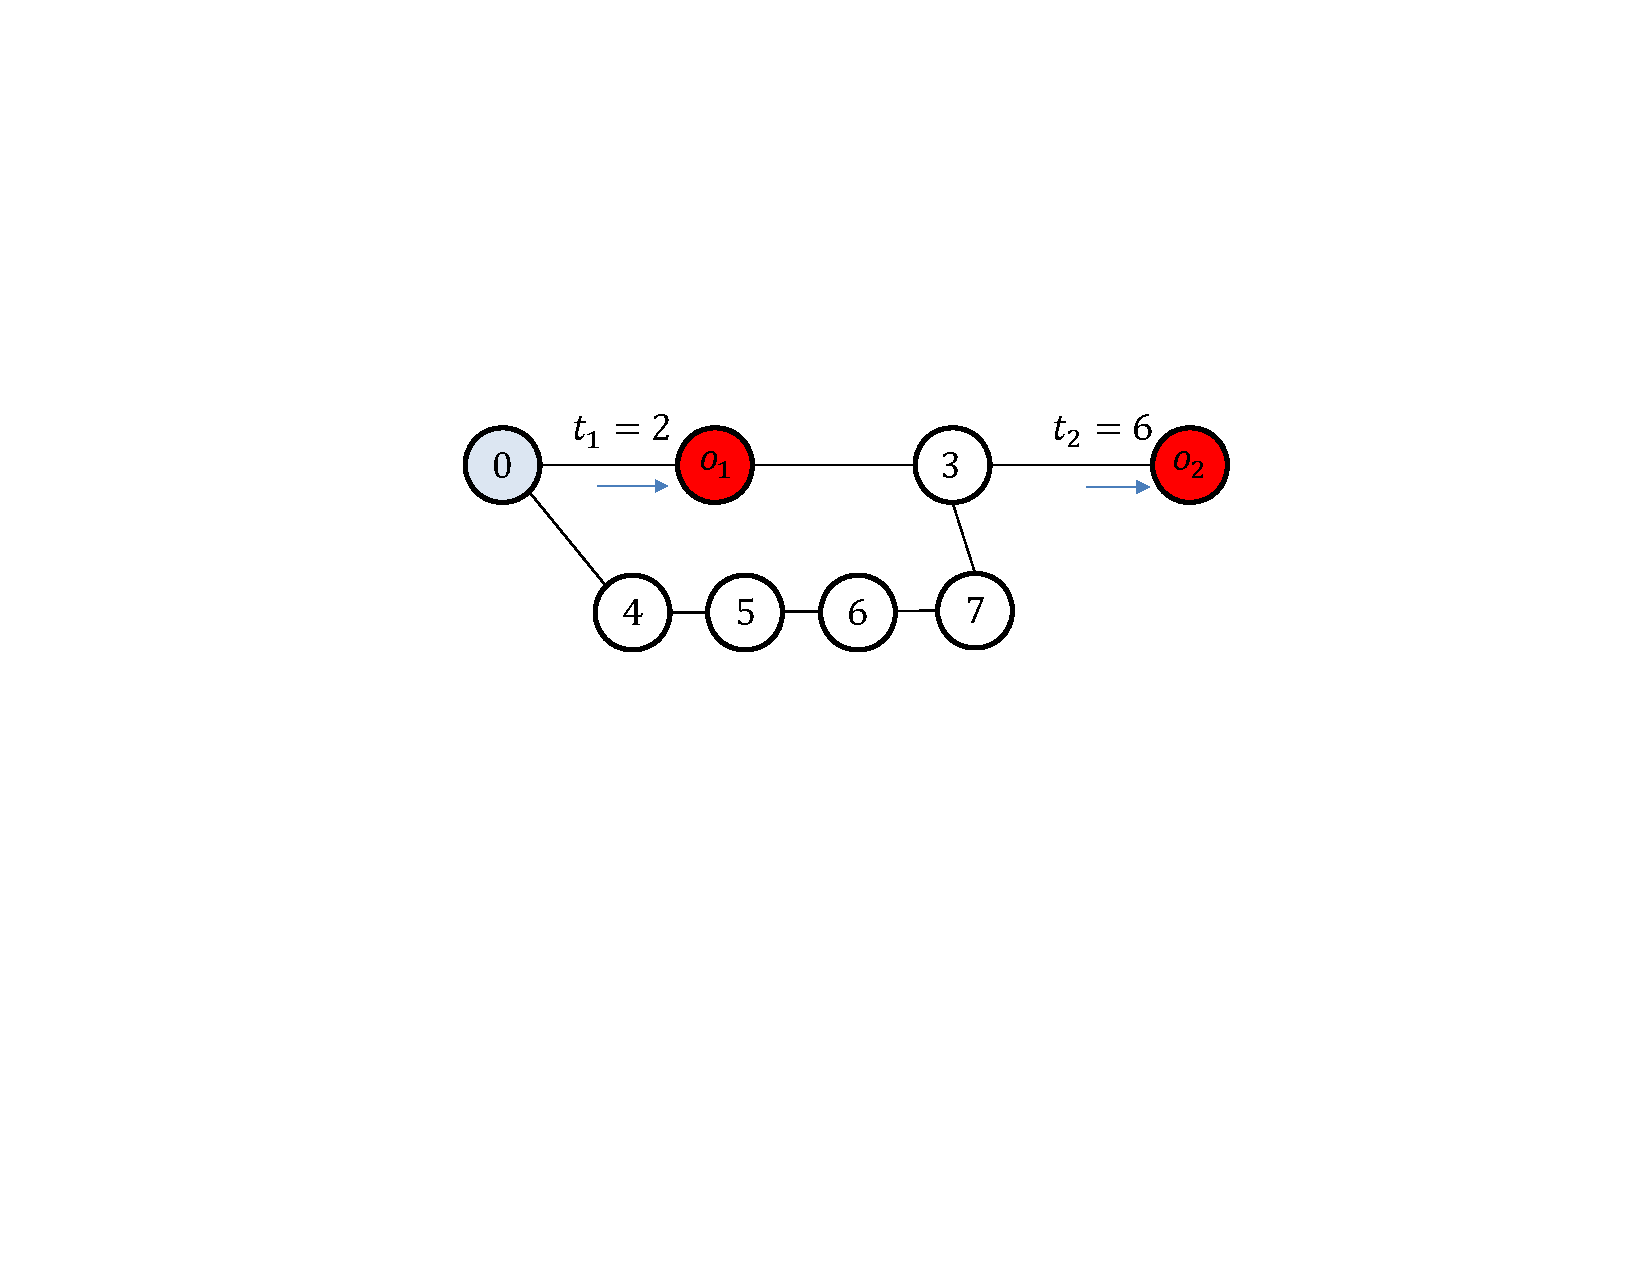
\includegraphics[width= 3in]{figures/pruning2}
\caption{The pruning used in \cite{pinto} can lead to false likelihood computations over loopy graphs; the scheme discounts the possibility of a spy passing the message to another spy.
%Delays $\theta_{ij}$ are modeled as Gaussians $\mathcal N(2,0.5)$, and spreading was run for 8 time units.
}
\label{fig:pruning2}
%\vspace*{-0.4in}
\end{figure}

\subsubsection{Trees}
We first tested the estimator on trees. As assumed in \cite{pinto}, each node transmits the message to its neighbors with an iid delay that is distributed according to $\mathcal N(2,0.5)$. Figure \ref{fig:pd_vs_spies} shows the probability of detection as a function of the fraction of spies over a 3-regular tree. We ran the simulation for 8 timesteps, leading to an average graph size of 75 nodes. Each datapoint is averaged over 4500 trials. Although \cite{pinto} does not provide simulation results over trees, we observe high detection probabilities for relatively low fractions of spies; with only 5 percent of the nodes spying, the source gets caught with probability 0.3. Note also that the ML estimator performs equally well with or without pruning (the plot lines are jittered to show both); this is because over trees, pruning never removes feasible candidates nodes or edges. We will see later that pruning over loopy graphs can remove feasible edges, and thereby impact the probability of detection. 
For reference, Figure \ref{fig:pd_vs_spies} also shows the probability of detection by the first-spy estimator. The ML estimator clearly outperforms the first-spy estimator, which is a good sanity check. Moreover, the first-spy estimator with pruning closely follows the theoretically-expected probability of detection; for a fraction of spies $p$, this probability grows as $P(\hat v=v^*)=1-(1-p)^d$ where $d$ denotes the degree of the underlying tree.
Figure \ref{fig:hops_vs_spies} shows the corresponding hop distances between the estimated source and the true source. We observe that with as few as 30 percent spies, this average hop distance is less than 0.1; the diameter of the graph is 8 hops. 
\begin{figure*}
  \begin{minipage}[c]{0.49\linewidth}
    \centering
    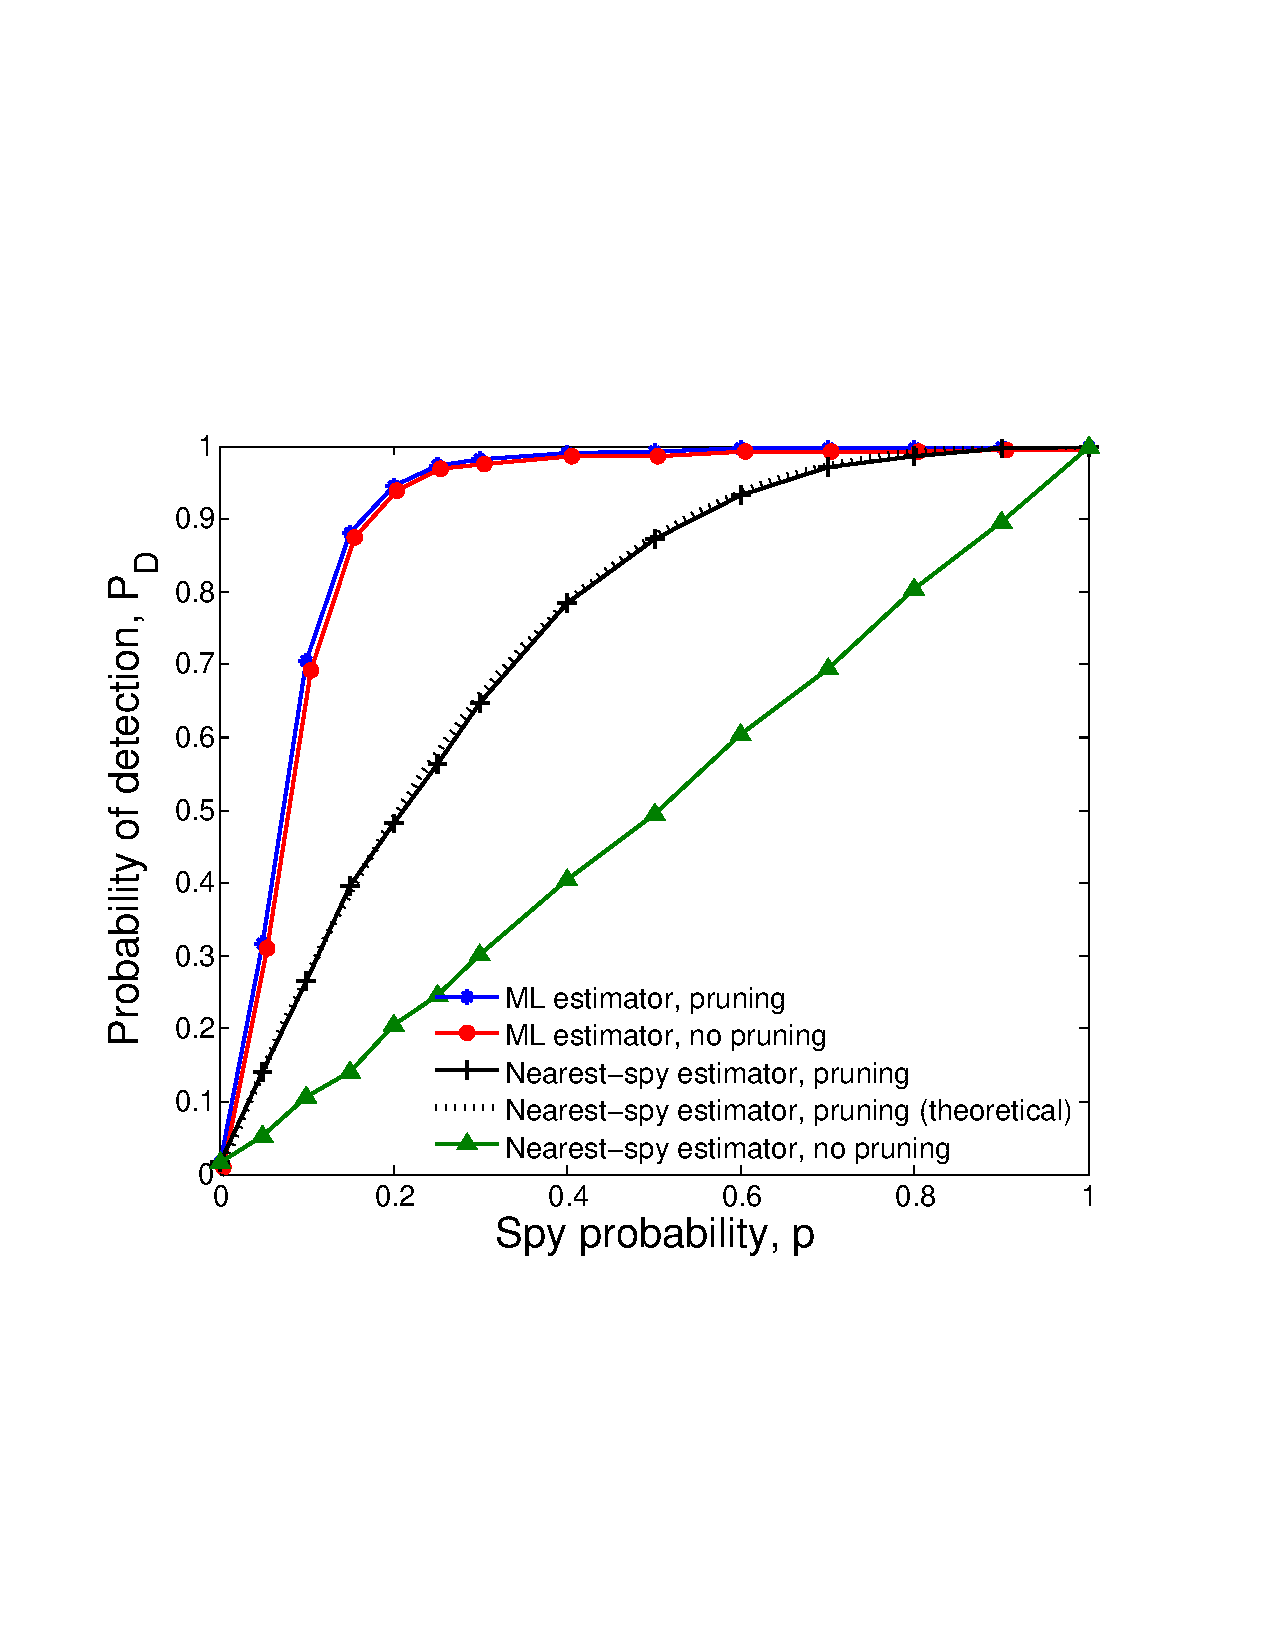
\includegraphics[width=0.9\linewidth]{figures/pd_vs_spies}
    \caption{Probability of detection, i.e. $P(\hat v = v^*)$, as a function of the spy probability $p$. This plot was generated over 3-regular trees. %Delays $\theta_{ij}$ are modeled as Gaussians $\mathcal N(2,0.5)$, and spreading was run for 8 time units.
    }
    \label{fig:pd_vs_spies}
  \end{minipage}
%\vspace*{-0.4in}
%\end{figure}
  \hfill
%\begin{figure}[ht]
  \begin{minipage}[c]{0.49\linewidth}
    \centering
    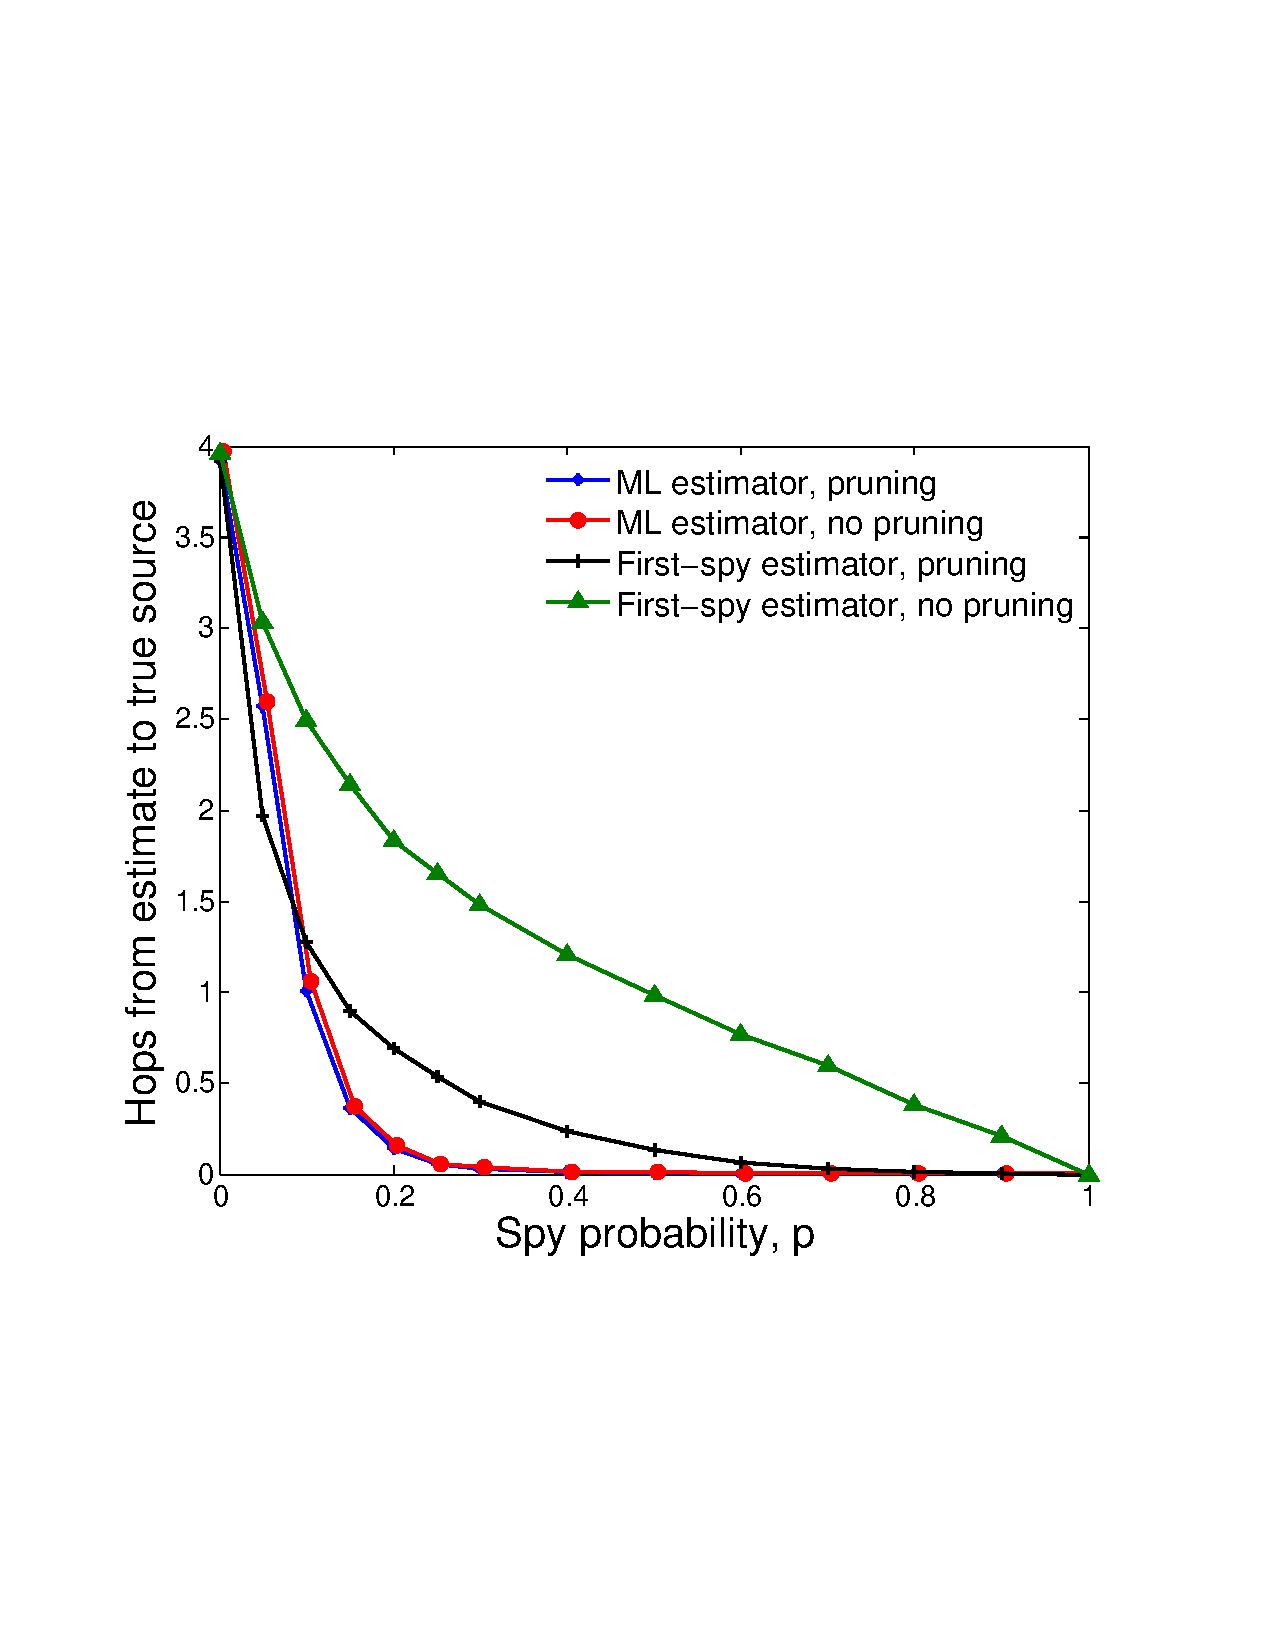
\includegraphics[width=0.9\linewidth]{figures/hops_vs_spies}
    \caption{Hop distance of the estimate $\hat v$ from the true source $v^*$ as a function of the spy probability $p$. This plot was generated over 3-regular trees. %Delays $\theta_{ij}$ are modeled as Gaussians $\mathcal N(2,0.5)$, and spreading was run for 8 time units.
    }
    \label{fig:hops_vs_spies}
  \end{minipage}
%\vspace*{-0.4in}
\end{figure*}

\subsection{Barabasi-Albert graphs}
We next considered random graphs with loops. \cite{pinto} considers a number of random graph structures, including Apollonian, Erdos-Renyi, and Barabasi-Albert. Due to time constraints, we only considered the latter. However, as mentioned earlier, we did not have access to the parameters used to generate the graphs in \cite{pinto}. To verify that we computed the estimator correctly, we considered a range of different parameters, and show that our results are at least plausibly consistent with the results provided in \cite{pinto}.

Figures \ref{fig:ba_graph} and \ref{fig:ba_graph_p1} show the probability of detection as a function of the fraction of spies for Barabasi-Albert graphs with $N=100$ nodes. We considered a minimum degree $m$ of 1 and 5. Each datapoint is averaged over 2000 trials. The figures illustrate that our numbers are at least plausible given the measurement provided in \cite{pinto}, albeit slightly low. Over graphs with a higher minimum degree (e.g., $m=6$), it seems entirely plausible that the optimal estimator could reach 90 percent accuracy with 41 percent spies. Unfortunately, each plot takes 24 hours to generate, and we ran out of time to test this hypothesis. However, given the estimator's strong performance on trees, we believe that our estimator implementation is consistent with that in \cite{pinto}. %It also gives the right numbers when we compute the likelihoods for small graphs by hand. 

\begin{figure*}[ht] \label{ fig7} 
  \begin{minipage}[b]{0.48\linewidth}
    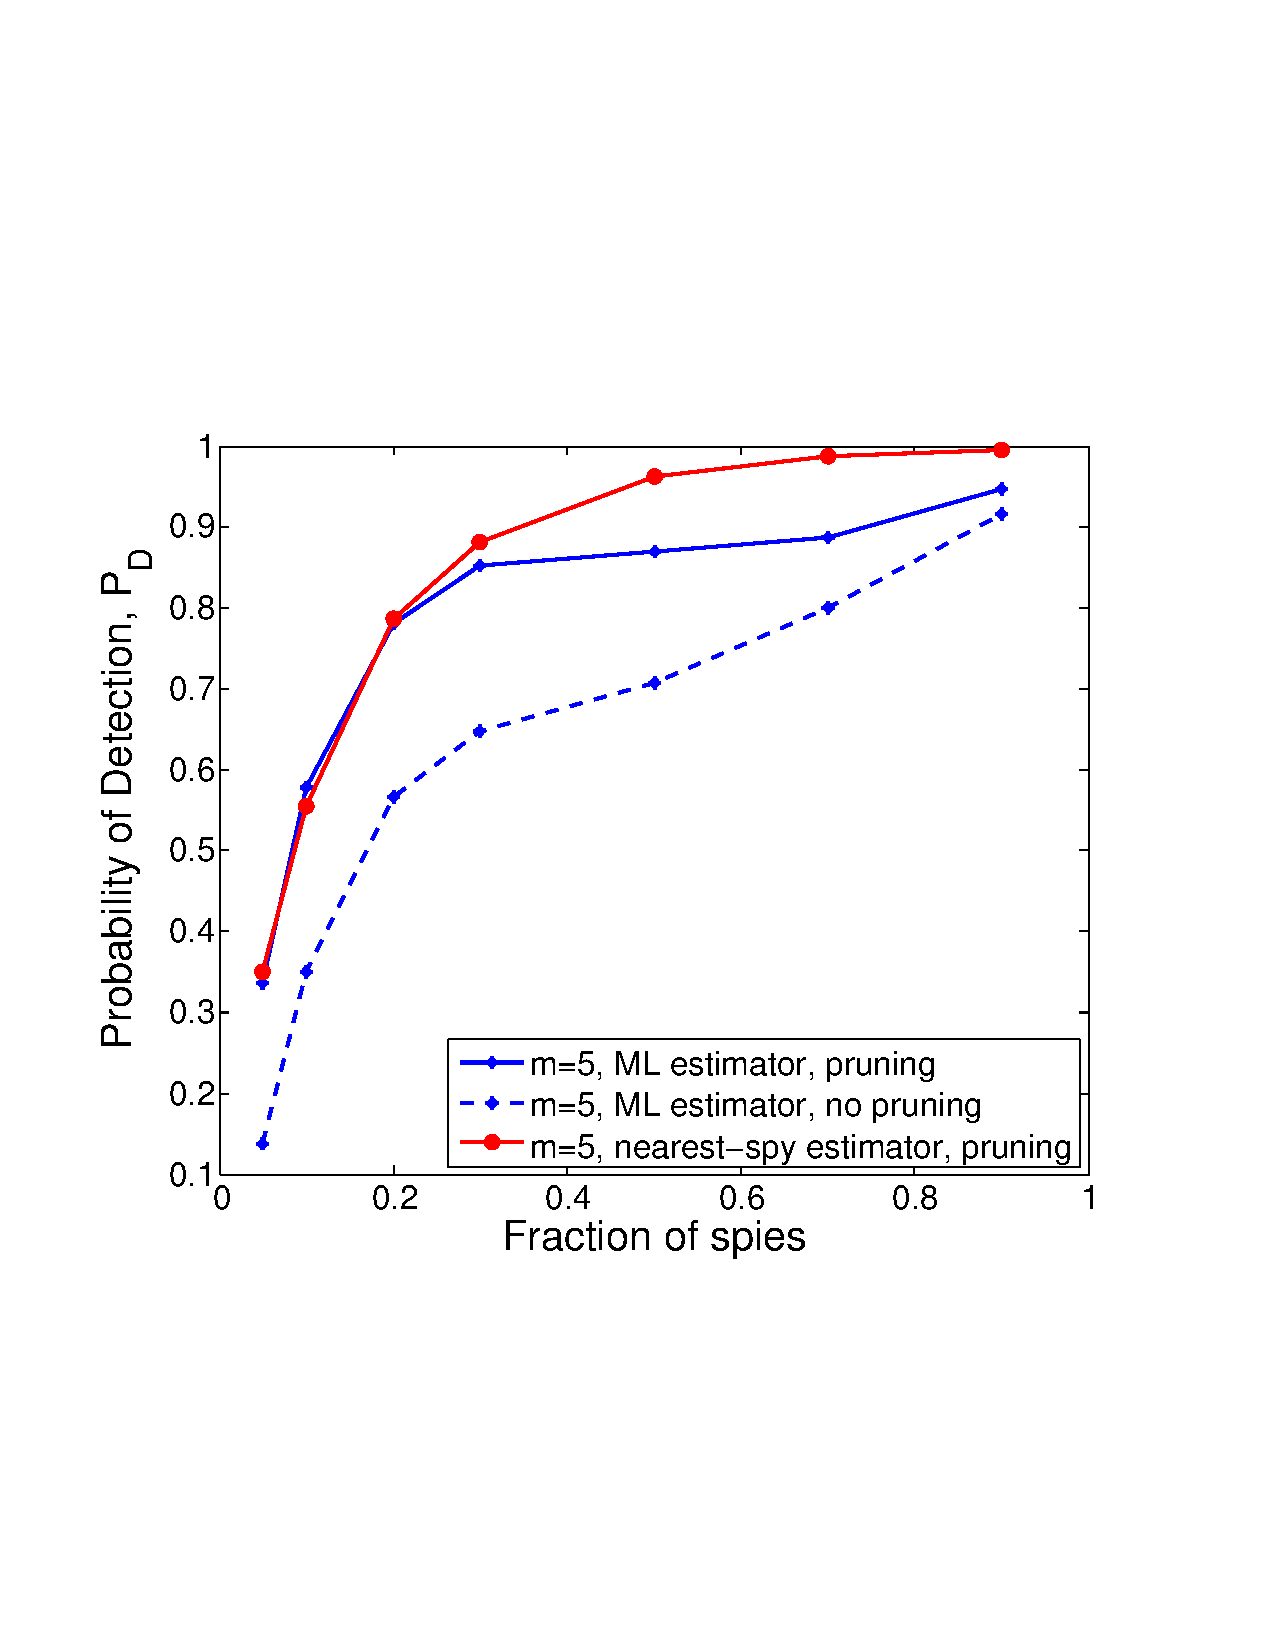
\includegraphics[width=3in]{figures/ba_graphs} 
    \caption{Probability of detection vs. spy fraction over Barabasi-Albert graphs with minimum degree $m=5$ and number of nodes $N=100$.} 
\label{fig:ba_graph}
  \end{minipage} 
\hfill
\begin{minipage}[b]{0.48\linewidth}
    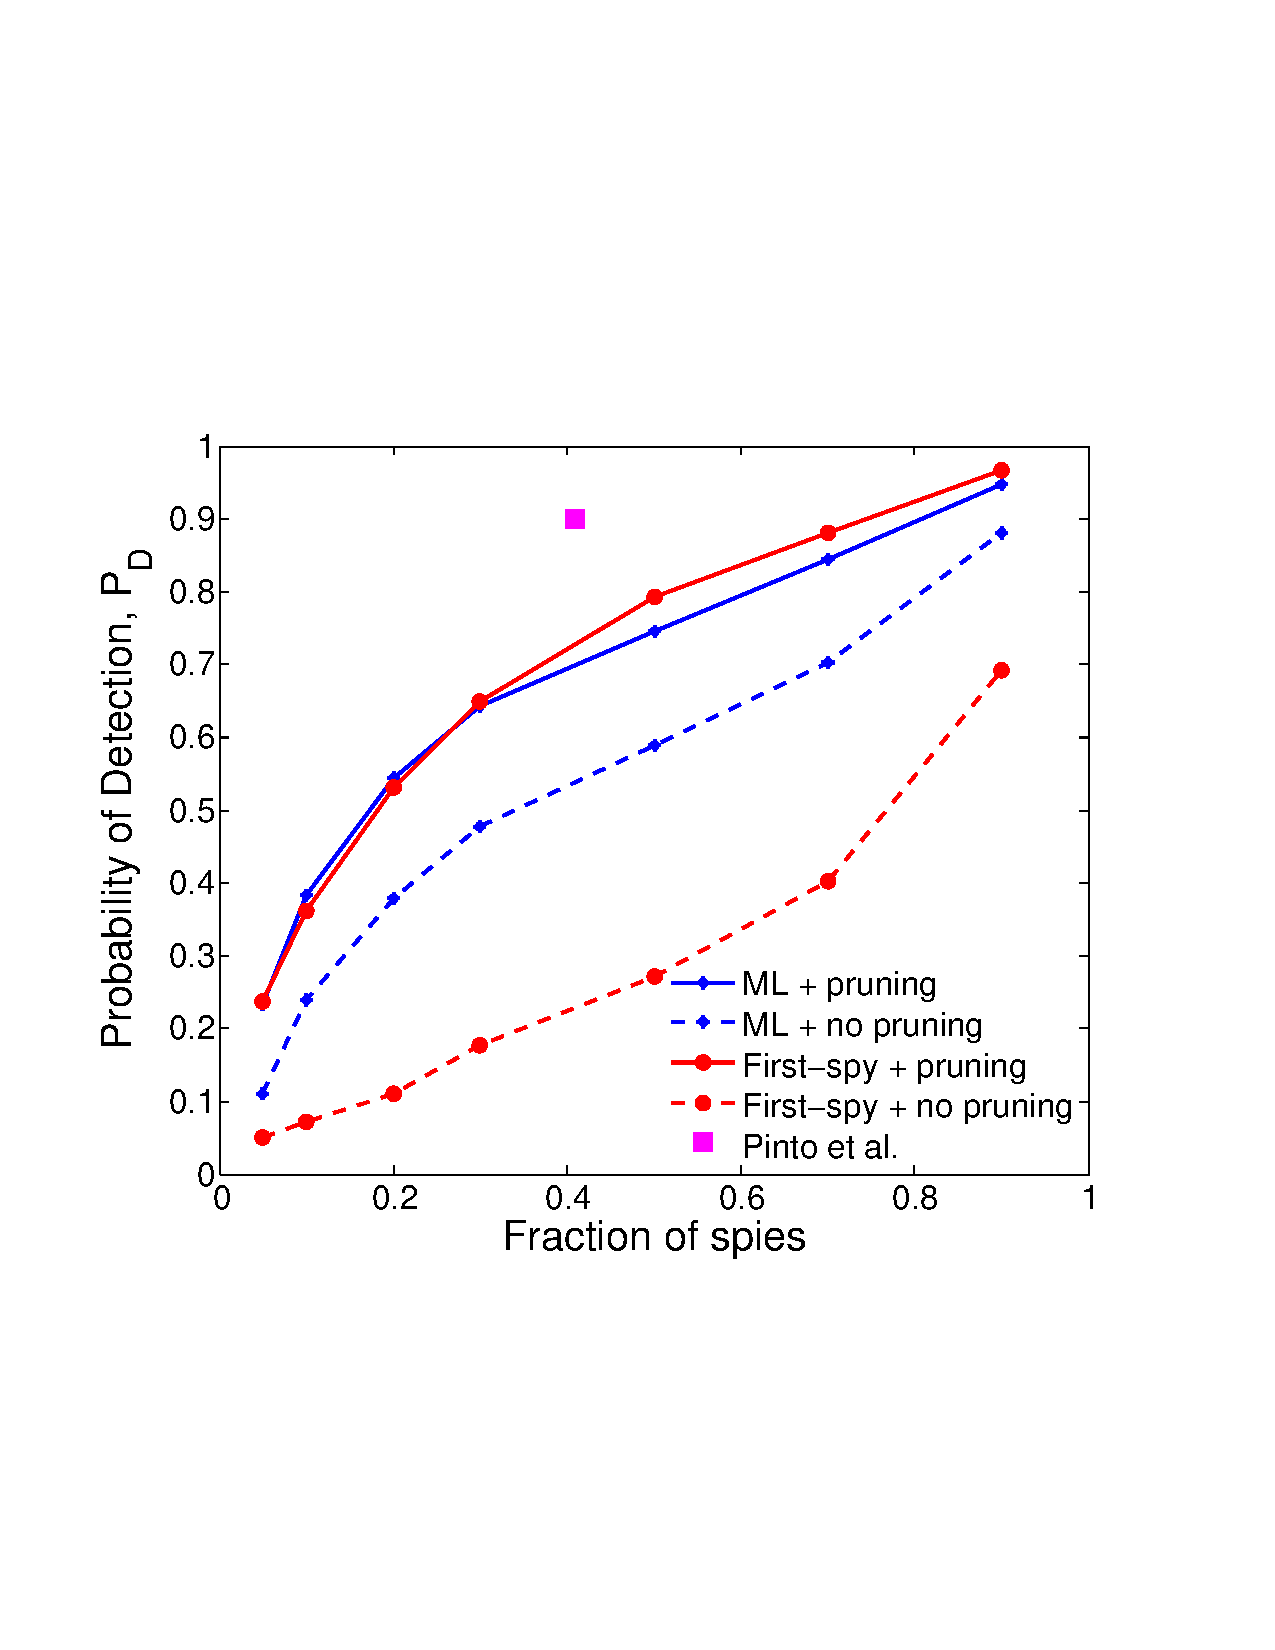
\includegraphics[width=3in]{figures/ba_graphs_p1} 
    \caption{Probability of detection vs. fraction over Barabasi-Albert graphs with minimum degree $m=1$ and number of nodes $N=100$.} 
\label{fig:ba_graph_p1}
  \end{minipage}
  \begin{minipage}[b]{0.48\linewidth}
    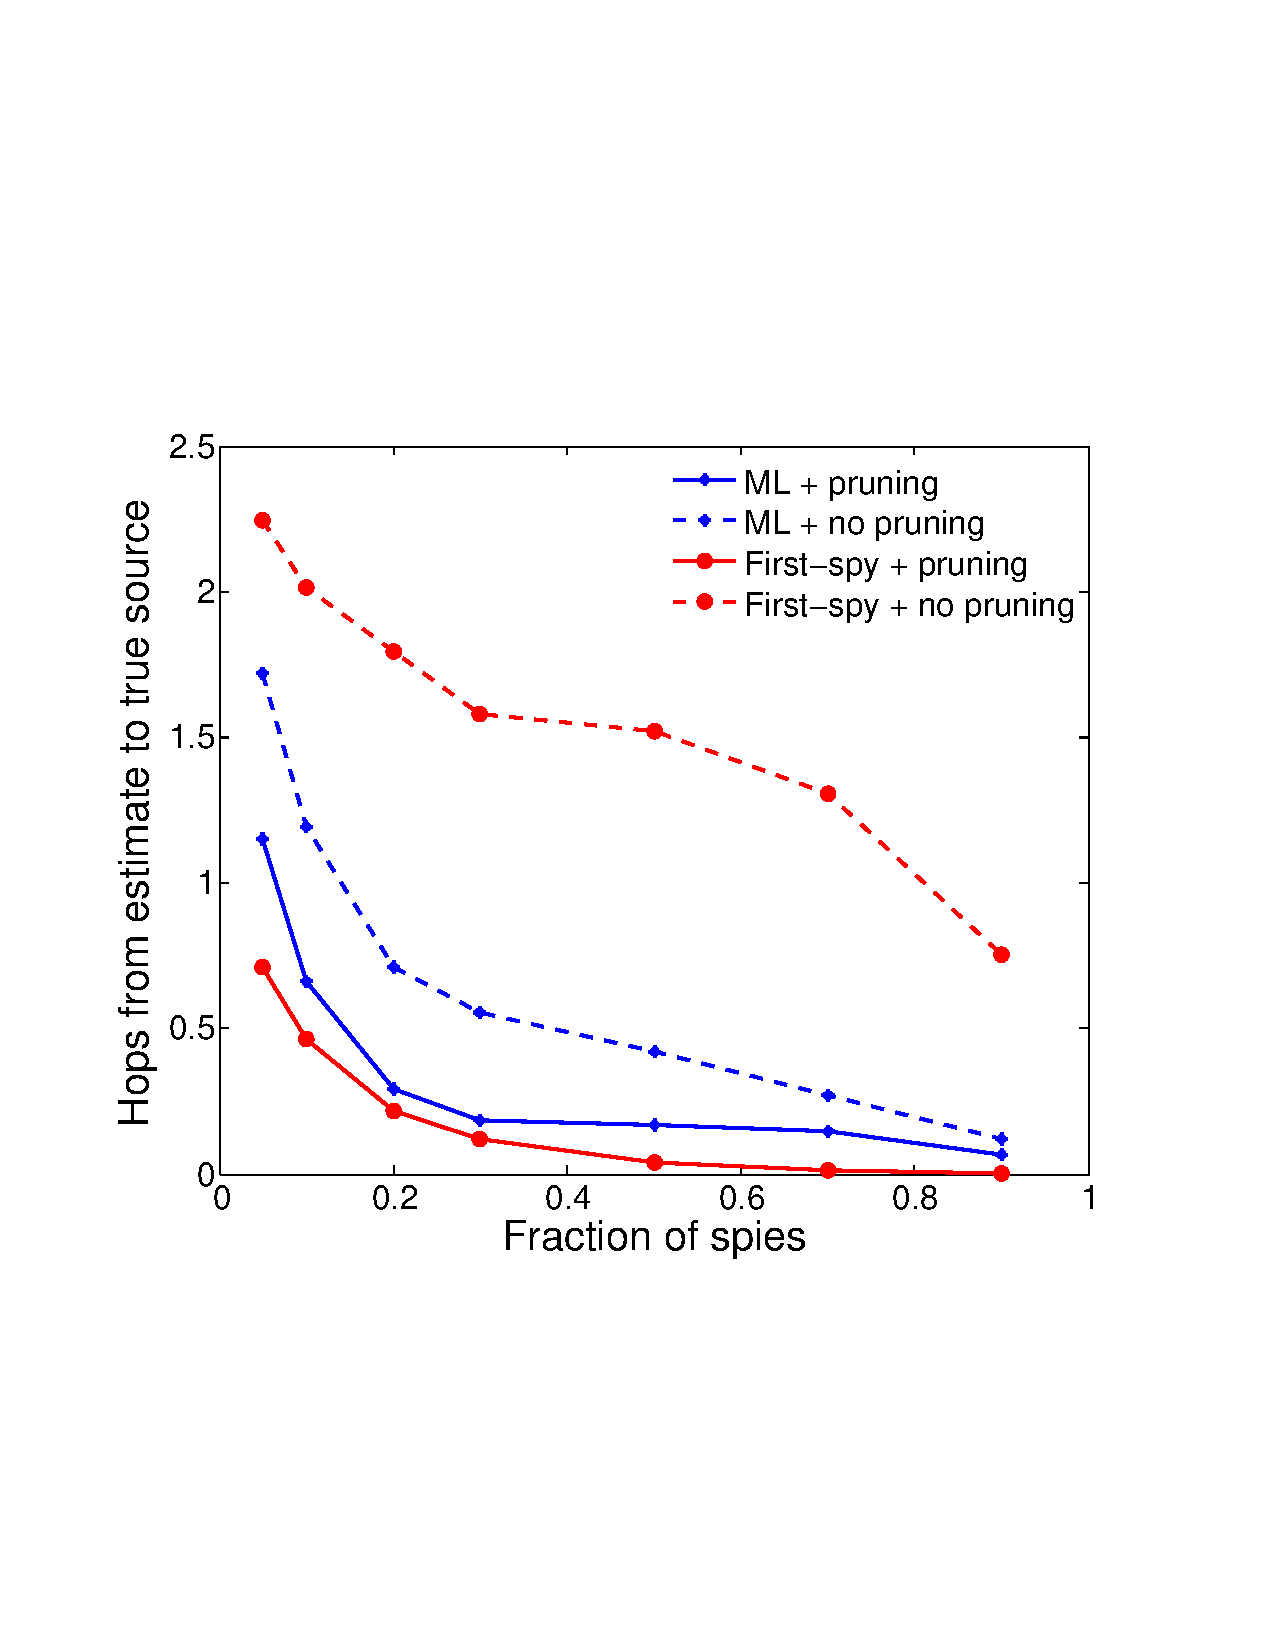
\includegraphics[width=3in]{figures/ba_hops} 
    \caption{Hop distance from estimate to true source vs. spy fraction over Barabasi-Albert graphs with minimum degree $m=5$ and number of nodes $N=100$.} 
\label{fig:ba_hops}
  \end{minipage} 
  \hfill
  \begin{minipage}[b]{0.48\linewidth}
    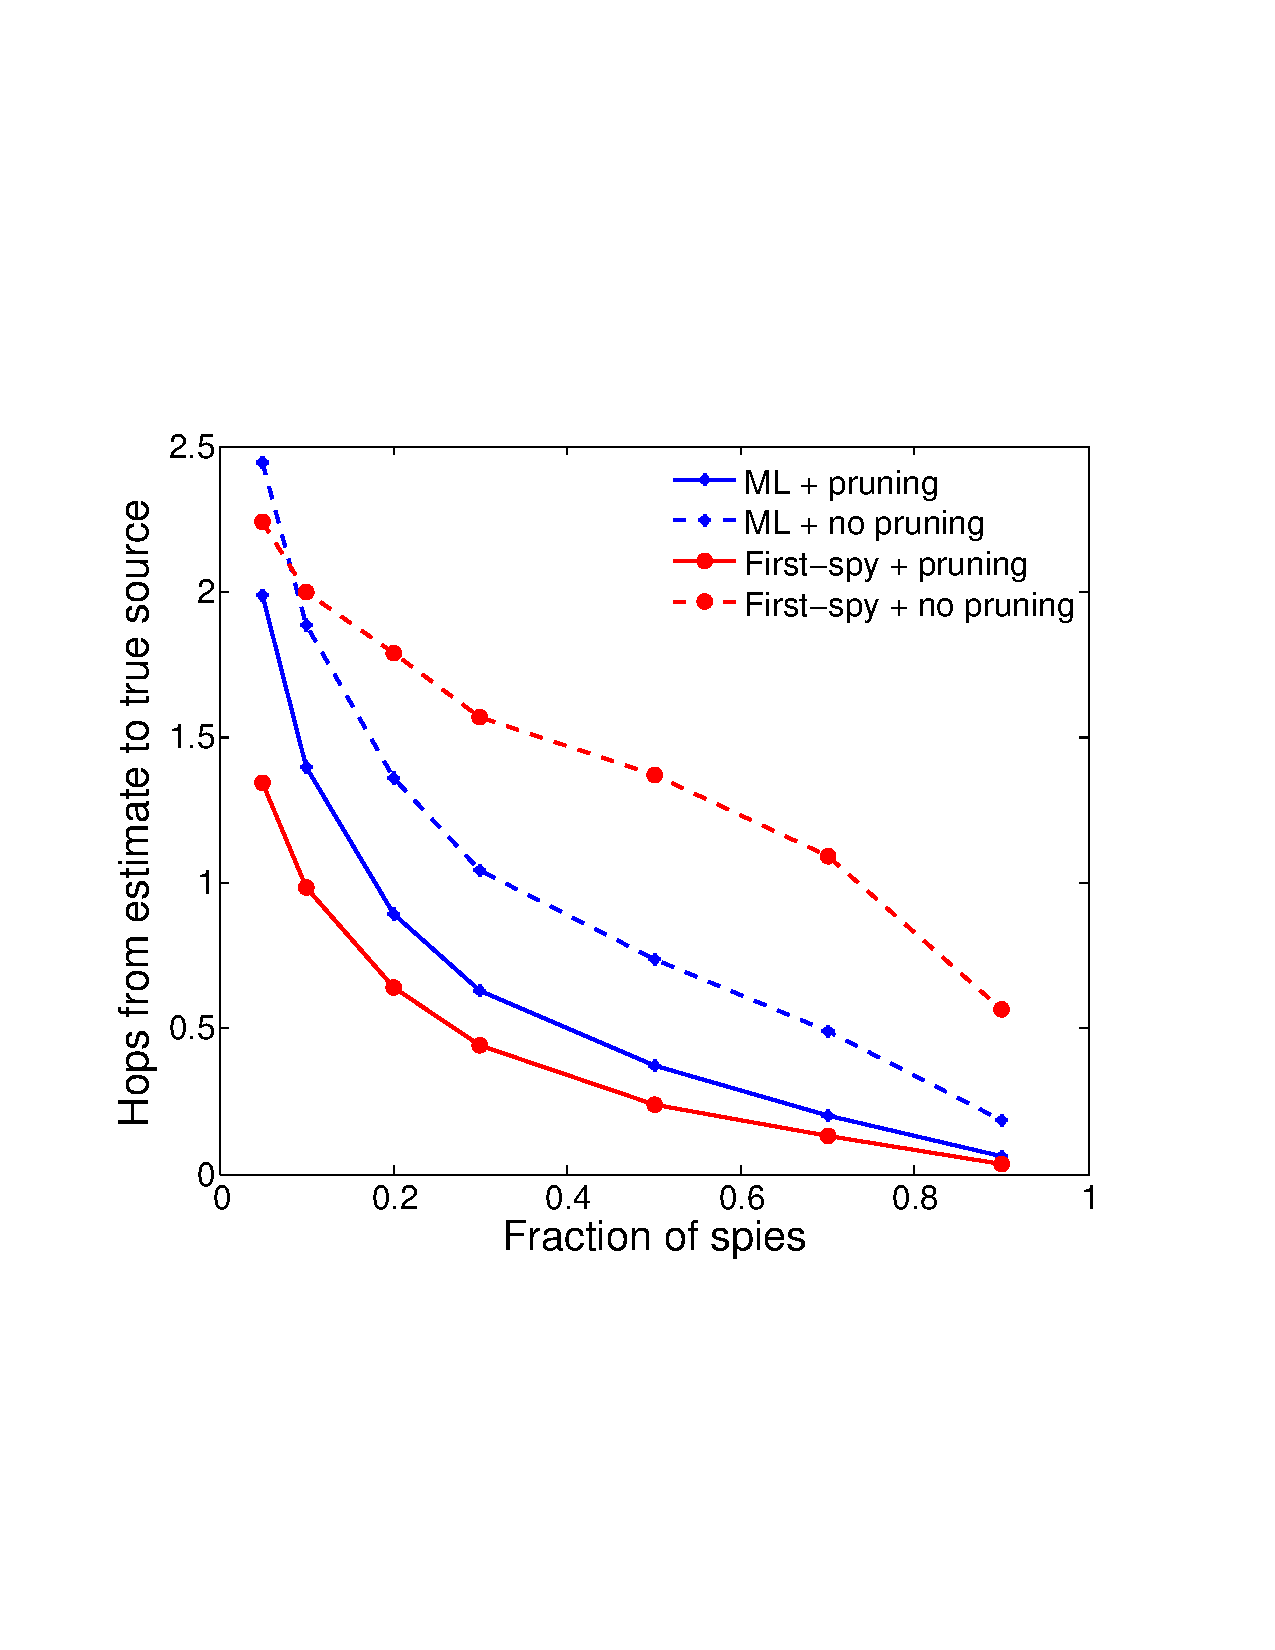
\includegraphics[width=3in]{figures/ba_hops_p1} 
    \caption{Hop distance from estimate to true source vs. spy fraction over Barabasi-Albert graphs with minimum degree $m=1$ and number of nodes $N=100$.} 
\label{fig:ba_hops_p1}
  \end{minipage} 
\end{figure*}

Note that the first-spy estimator with pruning performs as well or better than the `ML' estimator (which is not actually ML over general graph structures). Moreover, we visualized the pruned graph $\mathcal G_a$ for a number of graph+spy realizations and observed that $\mathcal G_a$ generally has very few honest nodes (about 10) when the fraction of spies is as small as 30; this pruned graph size only decreases as spy fraction increases. 
We want to highlight that the first-spy estimator with pruning always returns a node from $\mathcal G_a$ by construction.  Moreover, the first-spy estimator achieves comparable accuracy to the ML estimator with orders of magnitude less computation; the first-spy estimator has complexity $O(1)$ as compared to $O(N^3)$ for the ML estimator. As such, one of the main takeaways from our study is that when direction-of-infection information is available and the graph is not tree-structured, there is no reason to use the estimator from \cite{pinto}; the first-spy estimator will do as well or better, while using only a fraction of the computation. 

Conversely, when there is no direction-of-infection information, the first-spy estimator performs poorly compared the estimator from \cite{pinto}. Even the hop distances from the true source, illustrated in Figures \ref{fig:ba_hops} and \ref{fig:ba_hops_p1}, are significantly higher for the first-spy estimator without pruning. The Pinto \emph{et al.} estimator appears to be powerful even when there is no direction information available; this problem setting was not explored in their original paper. Indeed, in the paper's original setting of a disease outbreak, the sampled observers (i.e., the spies in our problem) are unlikely to know who infected them. As such, it is important to understand how these estimators perform without direction information. Unfortunately, this also implies that deanonymization may be feasible with only a small fraction of spy nodes---even when direction-of-infection information is unavailable.




\subsection{Facebook dataset}

Randomized graphs provide decent estimates for the estimators' effectivness, but they are still different from real datasets. In order to test our estimators on realistic data, we use a Facebook dataset~\cite{viswanath-2009-activity} from New Orleans. The dataset contains all of the user-to-user connections on Facebook in New Orleans as of 2008. Since the number of users is large, we take the first 800 nodes in the graph (the dataset orders the links) and construct a connected subgraph. We then use this subgraph to run our experiments by randomly choosing a propagation source. Because of limited time, we ran 30 trials for both 5\% and 15\% spy nodes. We believe that 15 percent is a conservative upper bound on the fraction of nodes that could plausibly be corrupted by bribing or coercing human participants; at their height, the Stasi employed 0.6 percent of the East German population as agents \cite{koehler1999stasi}. We do not consider the case where an adversary manages to infect devices with malware, in which case the fraction of spies could be significantly higher, and nodes might misbehave in unpredictable ways.

Table~\ref{table:fb:05} and table~\ref{table:fb:15} show the estimators' results for 30 trials with 5\% and 15\% randomly corrupted nodes. 

\begin{table}
\label{table:fb:05}
\begin{tabular}{c | c | c}
  & With direction & W/o direction \\
  \hline
  First spy & 30.00 \% & 0.00 \% \\ 
  Max Likelihood & 40.00 \% & 16.67 \% \\
\end{tabular}
\caption{Estimators' performance (percentage of accurate for 30 trials) on the Facebook dataset: 5\% random spies}
\end{table}


\begin{table}
\label{table:fb:15}
\begin{tabular}{c | c | c}
  & With direction & W/o direction \\
  \hline
  First spy & 66.67 \% & 3.33 \% \\ 
  Max Likelihood & 63.33\% & 26.67 \% \\
\end{tabular}
\caption{Estimators' performance (percentage of accurate for 30 trials) on the Facebook dataset: 15\% random spies}
\end{table}

\section{Discussion}

The results in \S\ref{sec:eval} suggest two main takeaway messages, which apply when the underlying graph is loopy and exhibits a power-law degree distribution:
\begin{itemize}
\item If the adversary has direction information for spy nodes, the first-spy estimator performs as well or better than the ML estimator, while using a small fraction of the computation.
\item If the adversary does not have access to direction information, the probability of deanonymization can decrease by as much as 50 percent, depending on the graph structure. In the absence of direction information, the ML estimator exhibits significantly higher deanonymization accuracy than the first-spy estimator.
\end{itemize} 

%There are various aspects of ML estimator that do not make sense algorithmically. 
%
%\begin{itemize}
%\item The estimator gives a log likelihood of 0 if a node $s$ is equidistant from all spy nodes, even if the timing information shows that $s$ is unlikely to be the true source. For example in Fig.~\ref{??}, we see that the ~~~~
%\end{itemize}

%There are some The estimator's pruning process is questionable. Given a graph $G$, the estimator prunes the graph using the direction of the propagation message. For every spy node $n_s$ that receives a message, the node prunes all edges that are not the propagation edge. After the pruning is done, the estimator discards all disconnected components except for the one containing the spy node with the earliest delay. After the pruning is done, the maximum likelihood estimator is run on the graph.
%
%This is pruning process is similar to the first-spy estimator, which picks a random neighbor that is closest to the 

The deanonymization rates reported in our plots and tables are upper bounds on what an adversary could achieve by selecting spy nodes uniformly at random. In our experiments, we assumed that nodes always `like' the message, so there is no asymmetry in the spread of the message. We also assumed that the adversary knows the entire graph structure, which may not be the case in practice. Nonetheless, our Facebook trials suggest that an adversary could plausibly deanonymize message senders with 10 percent accuracy by corrupting only 5 percent of nodes. This is a fairly high return on investment, and could be economically feasible for an adversary. 

We used a Gaussian propagation delay for all simulations, which may not be completely faithful to the delays observed in practice. However, this model is reasonable for small fractions of spies. As long as the per-edge delay random variable has finite moments, the sum of several such iid random variables will be well-approximated by a Gaussian due to the Central Limit Theorem. When the fraction of spies is low, pairs of spies will be a few hops apart on average, so the overall delay can be modeled as the sum of several delay random variables, i.e., approximately Gaussian. For this reason, we do not believe that our propagation model is a primary source of bias in our results---at least when the spy fraction is small.

Based on our findings, it could be useful to design a message-spreading algorithm that is specifically tailored to resist deanonymization attempts. For instance, instead of spreading the message symmetrically to a node's friends, perhaps the algorithm should only spread to a subset, and with some delay. The key here seems to be breaking the symmetry that is introduced by diffusion. 
\section{Future work}

Due to some major roadblocks in our project (mainly problems with the maximum likelihood estimator), we were not able to accomplish some of our original goals. 

\begin{itemize}

\item In the simulation, all nodes choose to ``like'' a message (unless it is a message that it has seen before). This is the best case scenario because the spy nodes are able to obtain the most amount of information. Thus, our simulation provides an upper bound on the source detection accuracy. The future work here would be to adjust the message propagation likelihood. The easiest parameter here is to change is for an honest node to \emph{probabilistically} like a new message: when an honest node $n$ receives a new message $M$, it ``likes'' $M$ with some probability $p$, and drops $M$ with probability $1-p$.

\item Spy node distribution is another parameter we want to adjust. In this paper, we used uniformly random distribution for spy nodes. This might not be a realistic estimate and in reality, one would expect some bias in the spy node sampling. For example, a political candidate may only be able to corrupt nodes that are closely related to him/her in the social network, therefore reducing the effectiveness of source detection. Another approach we can try here is similar to the one described in the paper: corrupting high degree nodes. Intuitively, this should give better accuracy because 1. with direction information, this node will get more accurate information 2. under the probabilistic propagation model, the node is more likely to receive messages. This is not such a realistic node because popular accounts are less likely to be hacked, but it will be an interesting case for comparison nonetheless.

\end{itemize}


% A category with the (minimum) three required fields
%\category{H.4}{Information Systems Applications}{Miscellaneous}
%A category including the fourth, optional field follows...
%\category{D.2.8}{Software Engineering}{Metrics}[complexity measures,
%performance measures]


%\terms{Systems}

%\keywords{ACM proceedings, \LaTeX, text tagging}





%
% The following two commands are all you need in the
% initial runs of your .tex file to
% produce the bibliography for the citations in your paper.
%% \bibliographystyle{abbrv}
%%     \bibliography{related_work,rp,rp-str,rp-conf}
% sigproc.bib is the name of the Bibliography in this case
% You must have a proper ``.bib'' file
%  and remember to run:
% latex bibtex latex latex
% to resolve all references

\bibliography{references}
\bibliographystyle{ieeetr}

%
% ACM needs 'a single self-contained file'!
%
%APPENDICES are optional
\balancecolumns

% That's all folks!
\end{document}

}
